% !TeX root = Bericht.tex
% !TeX spellcheck = de_DE
\section{Durchführung}

%\begin{figure}[H]
%    \centering
%    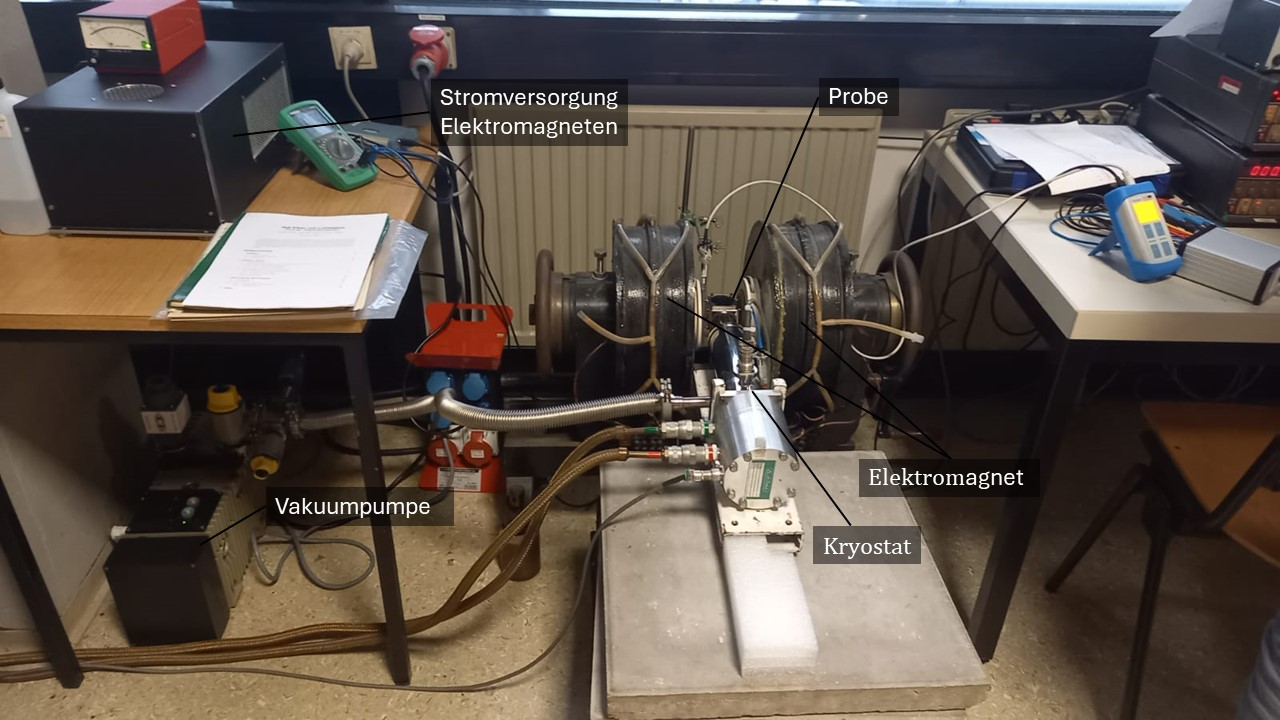
\includegraphics[width=\linewidth]{BildExberimentAufbauBeschriftung.JPG}
%    \caption{In dieser Abbildung sind der Kryostat, die Magnetspulen sowie die Sonde zur Messung des Magnetfeldes zu erkennen.}
%    \label{ExperimetAufbau}
%\end{figure}



Im Anschluss an die Installation des Zählrohrs wurde der Messaufbau mit dem Computer verbunden und das zugehörige Bedienungsprogramm gestartet. Der Aufbau ist in \autoref{aufbau_beschriftet} dargestellt. Zu erkennen ist auf der linken Seite der Draht, der durch Erhitzen durch Anlegen einer Anodenspannung und eines Stromflusses dazu gebracht wird, Elektronen zu emittieren. Durch die Blende kommen die Röntgenquanten in den rechten Raum des Geräts. Hier ist der schwenkbare Arm mit Winkelskala erkenntlich. Der Winkel wird relativ zur Horizontalen gemessen. Am Ende des Arms wird ein Geiger-Müller-Zählrohr befestigt, das mithilfe eines Kabels mit dem GM-Anschluss verbunden wird. Außerhalb des Geräts wird dieser Kabelanschluss mit dem Computer zur Datennahme verbunden. Am Gelenk des Schwenkarms befindet sich ein Steckplatz, auf dem ein Kristall zur Aufspaltung der Röntgenquanten in ihre Wellenlängen angebracht werden kann. 
\begin{figure}[H]
	\centering
	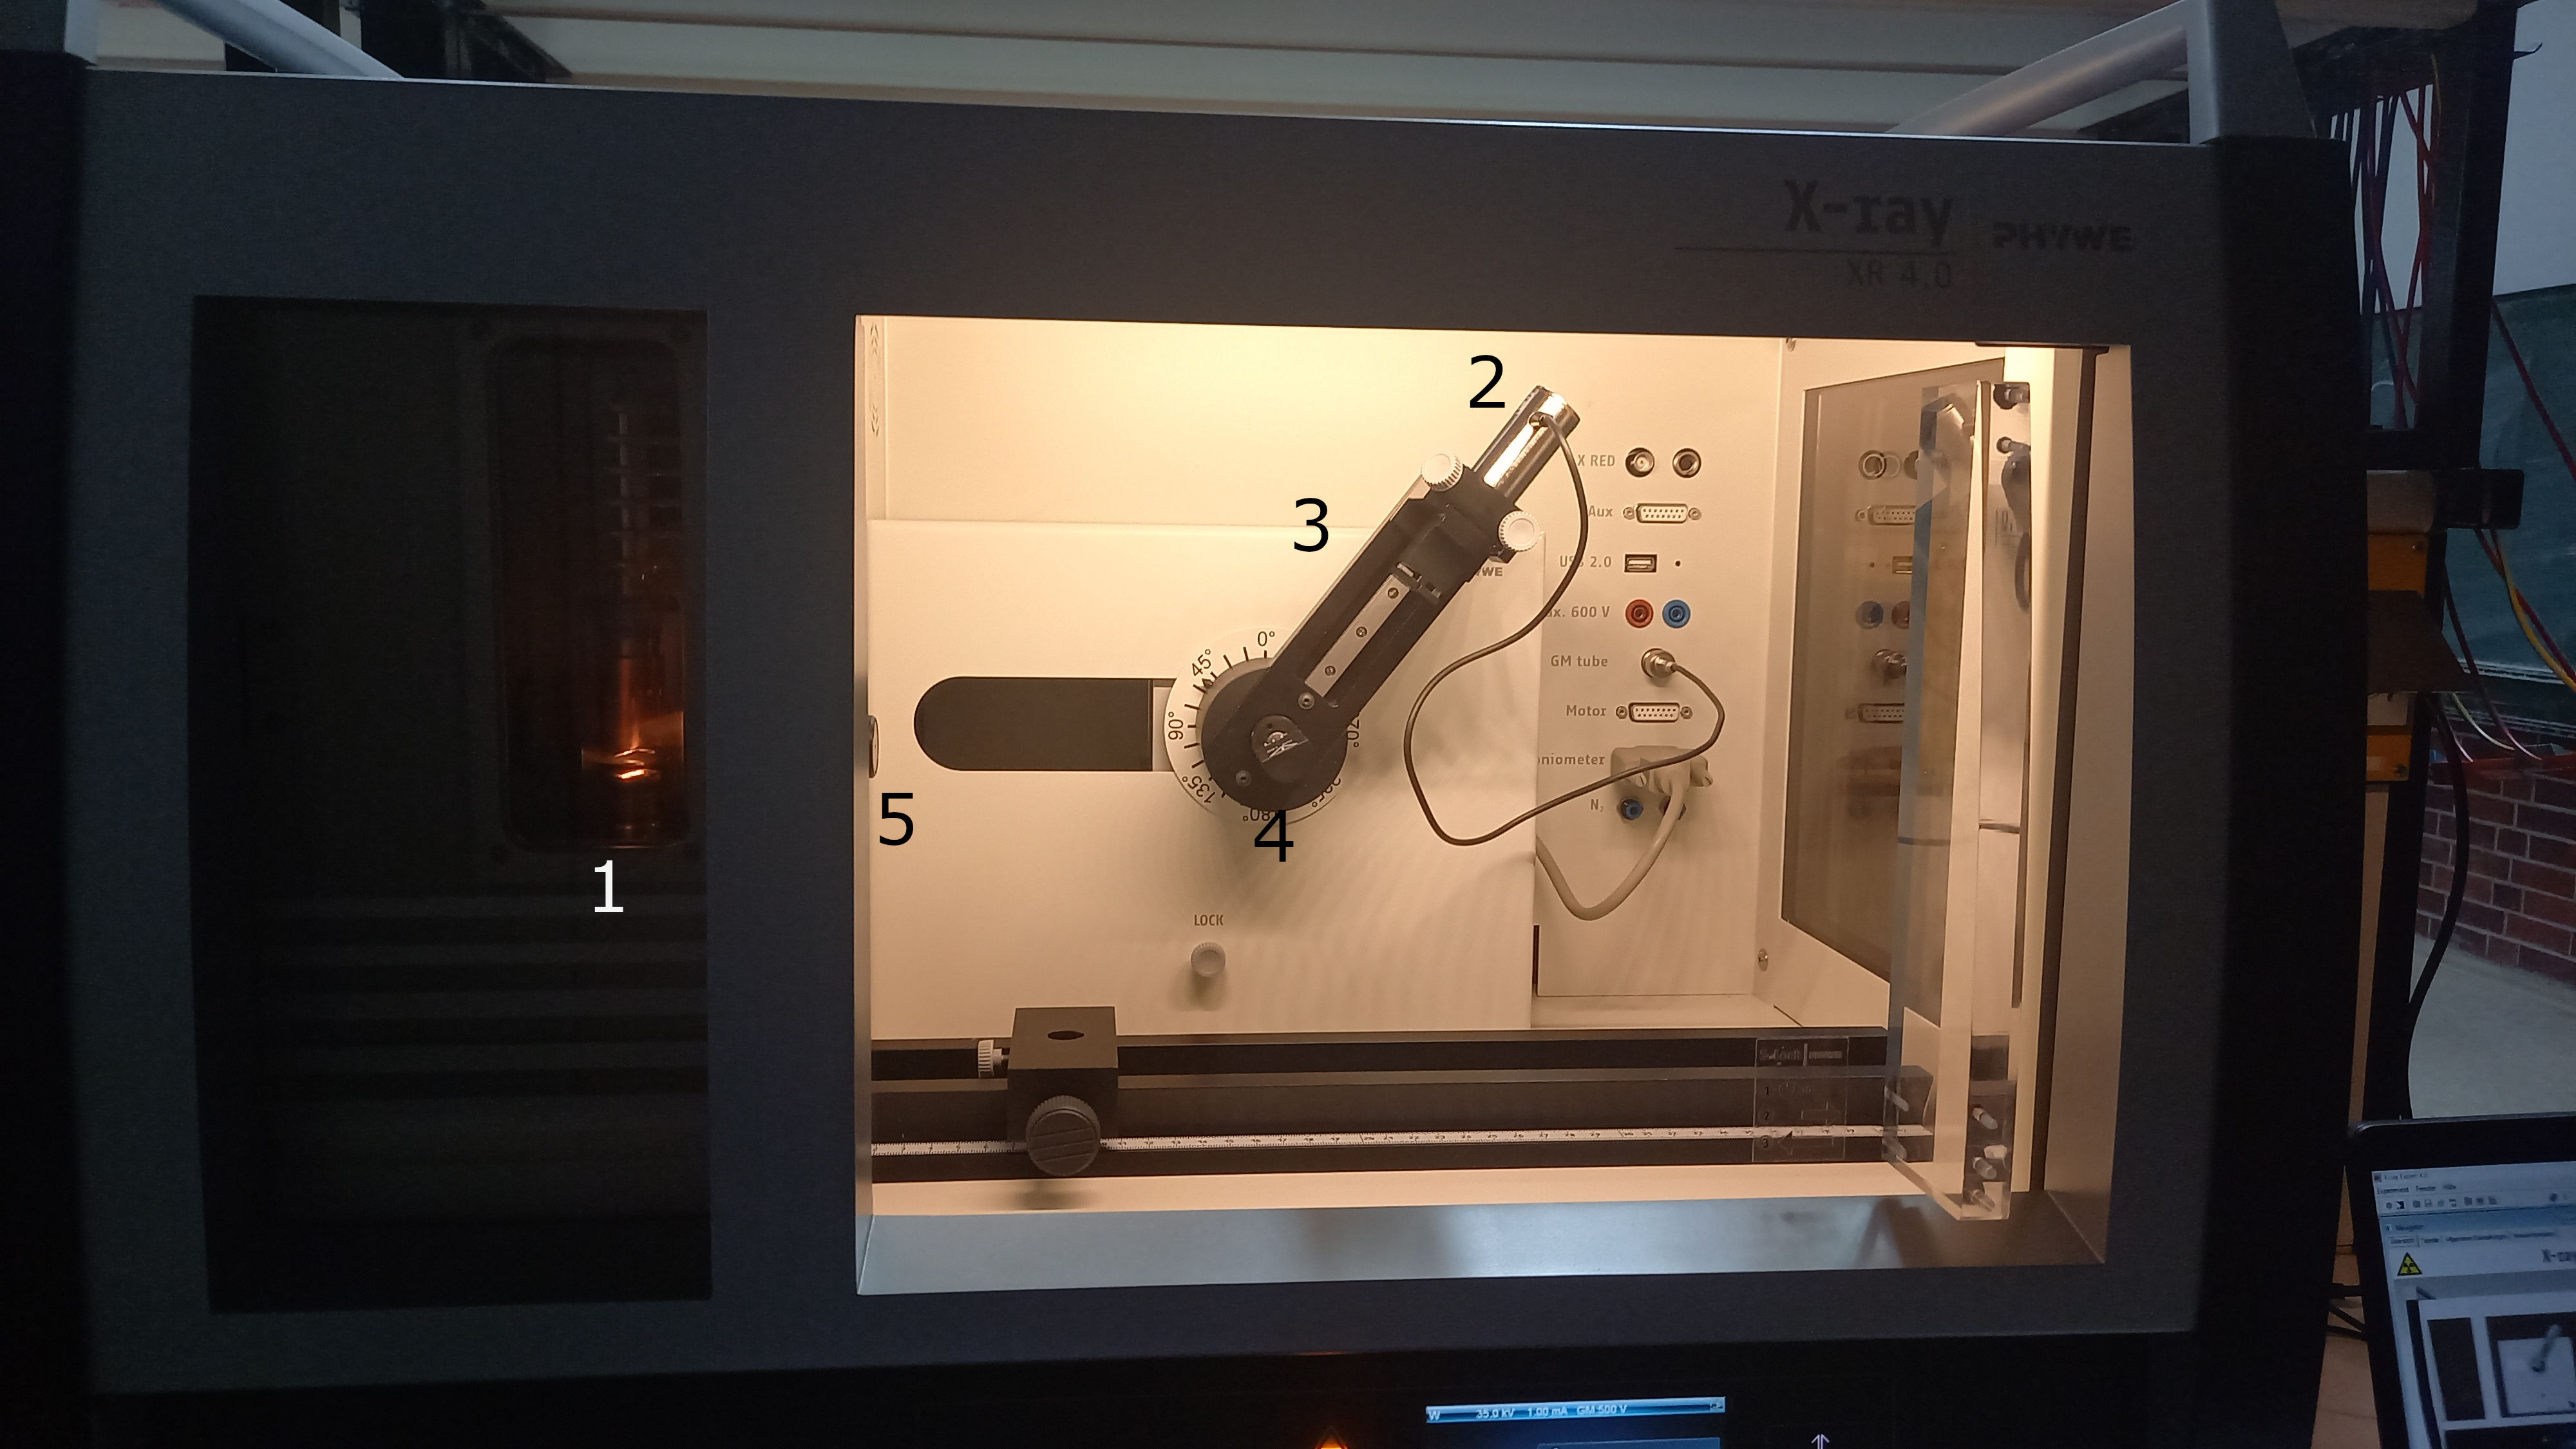
\includegraphics[width=\linewidth]{aufbau_beschriftet}
	\caption{Versuchsaufbau: 1) Anode für Elektronenemission 2) Geiger-Müller-Zählrohr 3) Schwenkbarer Arm mit Winkeleinstellung 4) Kristall 5) Blende.}
	\label{aufbau_beschriftet}
\end{figure}




\subsection{ Zählrohrcharakteristik}
Zur Charakterisierung des Zählrohrs wurde zunächst eine manuelle Sondierung durchgeführt, um die ungefähren Positionen der einzelnen Bereiche zu bestimmen. Dazu wurde der Winkel des Zählrohrs auf \ang{5.5} eingestellt, um eine Sättigung bei maximaler Zählrohrspannung von $500 \unit{V}$ zu vermeiden. Als Beschleunigungsspannung im Strahlungsemitter wurde $35 \unit{kV}$ bei einem Emissionsstrom von $1 \unit{mA}$ gewählt. Die Zählrohrspannung wurde dabei auf $500 \unit{V} $ gesetzt. Nach der Aussonderung wurde eine Schrittweite von 10 zwischen $300 \unit{V}$ und $310 \unit{V}$, von $1  \unit{V}$ zwischen $310  \unit{V}$ und $320 \unit{V}$, von $5 \unit{V}$ zwischen $320 \unit{V}$ und $350 \unit{V}$ und von $25 \unit{V}$ zwischen $350 \unit{V}$ und $500 \unit{V}$ gewählt. Der Grund hierfür ist, dass wir im am höchsten aufgelösten Bereich das charakteristische Ereignis untersuchen können und außerhalb dieses Bereichs ein konstanter Wert erwartet wird. Zu jedem Schritt der Zählrohrspannung werden drei angezeigte  Ereigniszahlen notiert. Da die Anzahl an Ereignissen auch bei konstanten Einstellungen zeitlich fluktuiert, werden für statistische Zwecke drei Werte pro Einstellung gemittelt. 

\subsection{Charakteristische Röntgenstrahlung}
Zunächst wurde der Kristall an der gewünschten Stelle eingebaut. Hierbei wurde ein LiF-Kristall (Lithiumfluorid) mit einer Gitterkonstante $d=201 \unit{pm}$ gewählt. Dieser Kristall wurde gewählt, da er die kleinste zur Verfügung stehende  Gitterkonstante aufwies, was eine feinere Auflösung der Wellenlängen ermöglichte. Die Winkelpositionierungsmöglichkeit des Versuchsaufbaus war auf den Wert \ang{0,1} beschränkt. Um eine automatisierte Messung vorzunehmen, wurde das Winkelverhältnis der Schwankung des Zählrohrs zur Schwankung des Kristalls auf 2 gesetzt. Das bedeutet, dass der eingestellte Winkel des Zählrohrs immer doppelt so groß ist wie der des Kristalls. Der Emissionsstrom wurde mit $I_\mathrm{Em}=1 \unit{mA}$ bei einer Beschleunigungsspannung von $U_\mathrm{Besch}=35 \unit{kV}$ bestimmt. Das Spektrum wurde zwischen \ang{5.5} und \ang {35.5} in Schritten von \ang{0.1} aufgetragen. Die Messung erfolgte an jedem Punkt für zwei Sekunden. Da auch Ereignisse berücksichtigt werden müssen, die nicht zuerst am Kristall gebeugt werden, wurde der gleiche Bereich unter den bekannten Parametern ebenfalls ohne den Kristall gemessen. 

\subsection{Bestimmung des Planckschen Wirkungsquantums}

Im Rahmen der Untersuchung war die kleinste emittierte Wellenlänge $\lambda_\mathrm{min}$ zu bestimmen. Zu diesem Zweck wurde zunächst der Anfangswinkel abgeschätzt, indem der Winkel manuell angepasst wurde, bis ein klarer Anstieg der Zählereignisse erkennbar war. Da bei steigender Spannung eine Verschiebung hin zu einer größeren Wellenlänge erwartet wird, wurde für jede Spannung extra sondiert. Die Messung wurde abgebrochen, sobald auf dem Bildschirm ein klarer Anstieg der Zählereignisse ersichtlich war. Es wurde darauf geachtet, dass eine hinreichende Anzahl an Messpunkten im Plateau vor dem Anstieg vorliegt, um eine Charakterisierung zu ermöglichen.  Die Messung wurde für Beschleunigungspannungen zwischen $15 \unit{V}$ und $30 \unit{V}$ in $2.5 \unit{V}$ Schritten durchgeführt. Der Emissionsstrom lag dabei bei $1 \unit{mA}$. 

\subsection{Absorptionsgesetz für Röntgenstrahlung}
%Hierzu wurden Aluminiumfolien mit den Dicken $0.02 \unit{mm}$, $0.04 \unit{mm}$, $0.06,  \unit{mm}$, $0.08 \unit{mm}$ und $0.1 \unit{mm}$ und Zinkfolion mit den Dicken $0.025 \unit{mm}$, $0.05 \unit{mm}$, $0.75 \unit{mm}$, $0.1 \unit{mm}$ und $0.1 \unit{mm}$. 

In diesem Teilversuch wird die Absorption von Röntgenstrahlen in Materie untersucht. Dafür wird die Zählrate bei Aluminium- und Zinkplatten unterschiedlicher Dicke gemessen. Diese Messungen werden für jeweils zwei Primär-Wellenlängen durchgeführt. Verwendet werden Aluminium-Folien mit den Dicken $0.02 \unit{mm}$, $0.04 \unit{mm}$, $0.06,  \unit{mm}$, $0.08 \unit{mm}$ und $0.1 \unit{mm}$. Bei den Zinkfolien betragen die Dicken $0.025 \unit{mm}$, $0.05 \unit{mm}$, $0.75 \unit{mm}$ und $0.1 \unit{mm}$. Die unterschiedlichen Wellenlängen werden durch Verändern des Winkels des GMZ realisiert, hierbei wurden die Winkel $ \ang{10.5}$ und $\ang{15}$ verwendet. 

Im zweiten Teil sollen die Massenabsorptionskoeffizienten für Aluminium-, Zink- und Zinnfolien konstanter Dicke in Abhängigkeit der Wellenlänge der Primärstrahlung bestimmt werden. Dabei wird eine der genannten Platten im schwenkbaren Arm platziert, und dann ein ganzes Spektrum aufgenommen. Dabei wird für Aluminium (Foliendicke $0.06 \unit{mm}$) der Winkel  von $\ang{10}$ bis $\ang{35}$ in Schritten von $\ang{0.5}$ gemessen. Für Zinn (Foliendicke $0.025) \unit{mm}$  von $\ang{10}$ bis $\ang{26.3}$ in Schritten $\ang{0.1}$ und für Zink (Foliendicke $0.05 \unit{mm}$) von $\ang{15}$ bis $\ang{22.8}$ in Schritten $\ang{0.1}$. Dabei wurden der Anfangswinkel so gewählt, dass der zu betrachtende Bereich aufgenommen wurde, danach wurde die Messung abgebrochen. Aufgrunddessen wirken die Winkel des Abbruches unerwartet bzw. unregelmäßig. Die Reduktion der Auflösung begründen wir mit der qualitativen Untersuchung des Verhaltens.  Selbes Verfahren wird danach auch für Kupferfolie, für Winkel von $\ang{5.5}$ bis $\ang{30.3}$, in Schritten von $\ang{0.1}$, und Nickelfolien, für  Winkel von $\ang{10}$ bis $\ang{26.3}$ in Schritten von $\ang{0.1}$ angewandt, um deren Absorptionskoeffizienten zu ermitteln. Diese beiden Folien waren $0.025 \unit{mm}$ dick. 